\part{Présentation et objectifs}
\chapter{Présentation du projet}
\subsection{Contexte}
De nos jours, les smartphones disposent tous d'une puce GPS permettant leur géolocalisation à chaque instant avec une précision de plus en plus grande. C'est donc l'outil idéal pour les joggers et cyclistes qui souhaitent enregistrer et analyser leurs performances. De nombreuses applications ont ainsi vues le jour ces dernières années pour répondre à ces besoins. On peut notamment évoquer le leader sur le marché des applications mobiles dans la catégorie santé et remise en forme qu'est Runtastic ou encore RunKeeper.\\

\begin{img}
  \includegraphics{img/Runtastic.png/image}
  \caption{Application Runtastic}
\end{img}

\begin{img}
  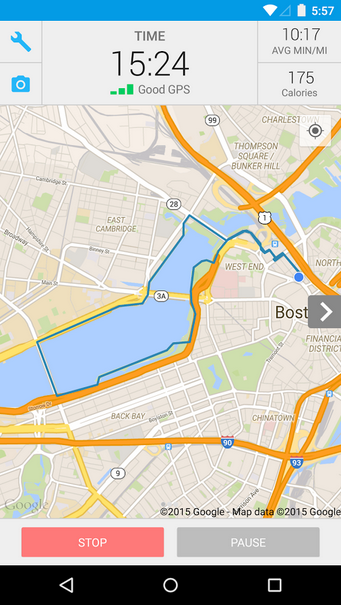
\includegraphics{img/Runkeeper.png}
  \caption{Application RunKeeper}
\end{img}

C'est dans ce contexte que notre tuteur, M. Mathet nous a proposé de concevoir et de développer une application mobile permettant d'enregistrer les tracés GPS des parcours de l'utilisateur et d'analyser ses performances. Mais aussi, et c'est ici que tous l'enjeu du projet se situe, de comparer en temps réel les performances de l'utilisateur par rapport aux  précédentes effectuées sur le même parcours. Concrètement, il s'agit d'afficher l'avance ou le retard en secondes qu'il a par rapport à une performance définie (la meilleure ou la moyenne des dernières). 

